{
Hypotesen for dette eksperiment er at det gyldnesnit ikke bliver brugt
mere end andre snit.
\subsection{Eksperimentsopstilling}
I \ref{chap:chap_afproevning} er de optimale tærskelværdier fundet.
Idet denne hypotese blot kigger på frekvensen for brug af det gyldnesnit
mod andre snit, hvis eneste restriktion er at de skal have et fælles
forhold til det gyldnesnit.
Det er også fordelagtigt at maksimere antallet af andre snit, da det
giver et bedre grundlag for eksperimentet.
Afstanden mellem to snit er begrænset af margin defineret til at være
$2.4\%$\ref{margin}. 
Denne margin skal være tilstede på begge sider af et snit, så derfor vil
hvert snit fylde $(2.4*2)\%$.
Det maksimale antal af snit på et billede må altså være
$100/4.8=20.833$. Hvilket ses på denne figur \ref{snitogmargin}
\begin{figure}[h!]
	\begin{center}
		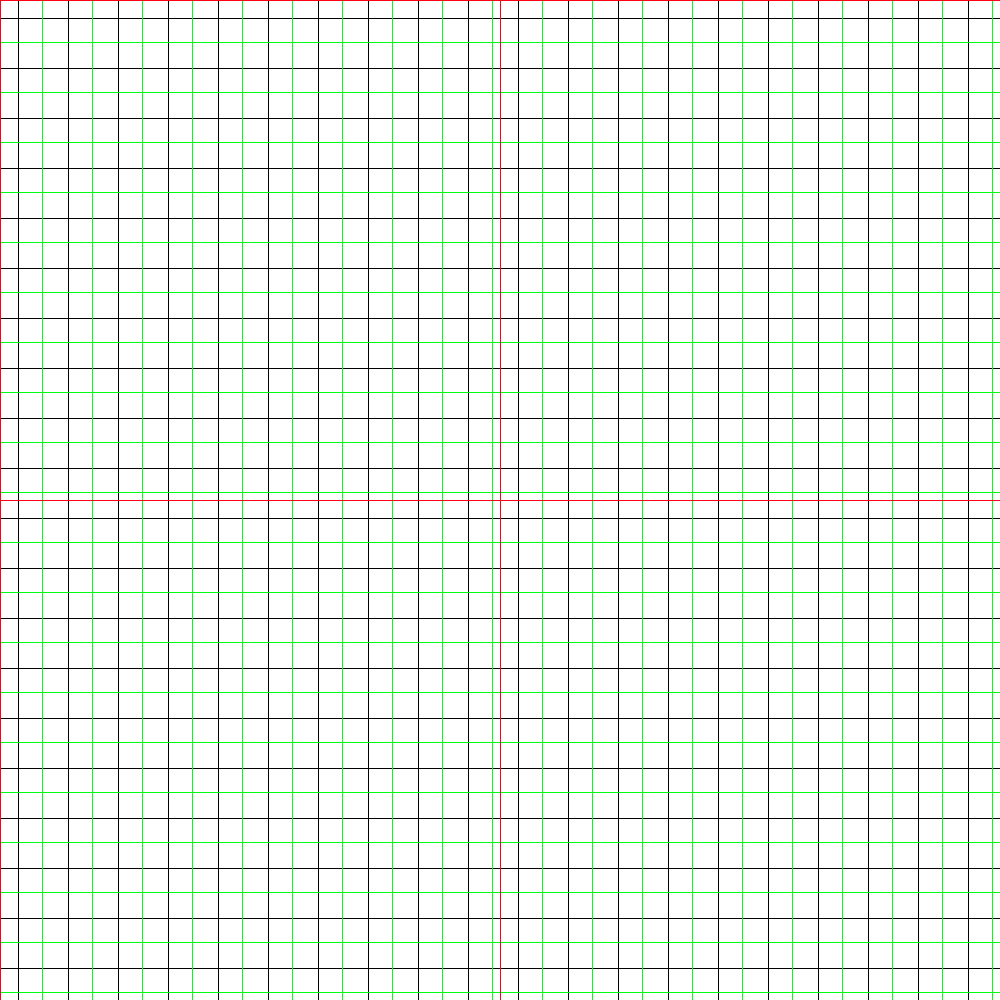
\includegraphics[scale=0.3]{afsnit/resultater/billeder/20_cuts_med_margin}
	\end{center}
	\caption{Sort:snittene, grøn: margins og rød er midten}
	\label{snitogmargin}
\end{figure}
Yderpunkterne $0.958$ og $0.518$ er problematiske, $0.958$'s margin
løber udover billedet, dvs. at den ren principielt går glip af at
detektere en masse interessante regioner.
$0.518$ lider af det modsatte problem, den kan potentielt fange
interessante regioner, på begge sider af midten.
For at være helt præcis så er det i $0.518$ tilfælde:\\
$1-0.518 = 0.482$
$0.518-0.482=0.036$\\
Hvilket er afstanden mellem de to snit.
Der er altså en stimmel på $0.05-0.036 = 0.014 = 1.4\%$ af billedet,
hvor interessante regioner bliver talt to gange.

Eksperimentet bliver kørt på alle 17364 billeder.
\newpage
\subsection{Forventninger}
Eftersom dette er det første større forsøg med den naive algoritme, er
forventningerne at alle snit med undtagelse af de to yderste snit
stortset indeholder samme antal interessante regioner.

\subsection{Resultater}
Resultaterne strider ikke mod hypotesen, dog tegner \ref{diffratios}
et meget et interessante billede. Det er kun de to snit der ligger
tættere på midten, der indeholder flere interessante regioner.
Antallet af interessante regioner stiger forholdvis konstant mellem
$0.77$ og op til $0.57$.

Med den nuværende algoritme og billedebase burde det gyldnesnit
altså ligge mellem $0.56803398875$ +- 2.4.
Og tyder meget på at midten langt mere er stedet kunstrene arbejder
ud fra.
%Indsæt graf over de forskellige ratios her.
\begin{figure}[h!]
	\begin{center}
		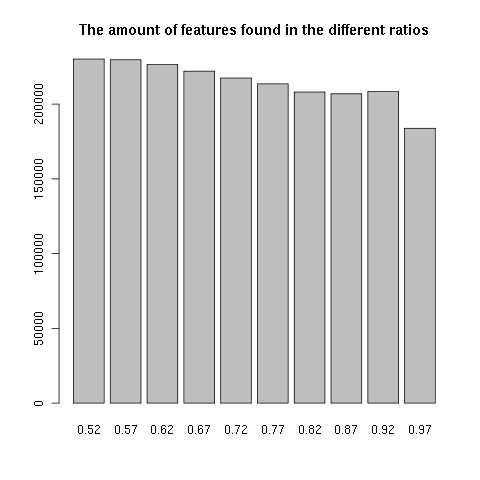
\includegraphics[scale=0.5]{afsnit/resultater/billeder/featsperratio.png}
	\end{center}
	\caption{Antal af detektere interessante regioner på de forskellige snit.}
	\label{diffratios}
\end{figure}


%\begin{verbatim}
%number of features in the golden ratio in different periodes
%
%{'1301-1350\r\n': 151894, '1551-1600\r\n': 184246, '1201-1250\r\n': 419, '1851-1900\r\n': 15092, '1101-1150\r\n': 2817, '1651-1700\r\n': 171119, '1351-1400\r\n': 35464, '1251-1300\r\n': 11864, '1451-1500\r\n': 428338, '1701-1750\r\n': 115703, '1151-1200\r\n': 14688, '1751-1800\r\n': 67703, '1801-1850\r\n': 79182, '1601-1650\r\n': 273832, '1401-1450\r\n': 199989, '1501-1550\r\n': 394100}
%Which golden ration is the most popular, ranging from 0 to 3
%[56092, 57044, 59181, 54152]
%features in the different ratios
%{0.66803398874999997: 222018, 0.86803398875000004: 206899, 0.56803398875: 229650, 0.96803398875000002: 183833, 0.76803398874999995: 213570, 0.91803398874999997: 208340, 0.81803398875: 208081, 0.71803398875000002: 217432, 0.51803398874999995: 230144, 0.61803398875000004: 226462}
%Top 10 cuts, where the most features was found
%[239, 250, 254, 257, 274, 288, 298, 326, 430, 436]
%Top 10 images
%[546, 552, 554, 569, 570, 578, 592, 616, 634, 675]
%Top 10 images, with only the features in the golden feature
%[73, 75, 76, 77, 78, 86, 87, 87, 99, 147]
%Top 10 images, with only features in 2/3 that counts
%[144, 146, 171, 204, 209, 211, 221, 228, 251, 300]
%\end{verbatim}
%TODO:tilføj en ud af hvor mange billeder der var i den periode!
%	og hvilke billeder der er i top 10!
%	og en fordelen af hvor mange features der er i billeder generelt.
%
}
% vim: set tw=72 spell spelllang=da:
